\begin{figure*}[t]
\centering
\small
\begin{minipage}{\linewidth}
    \begin{minipage}{0.3\linewidth}
        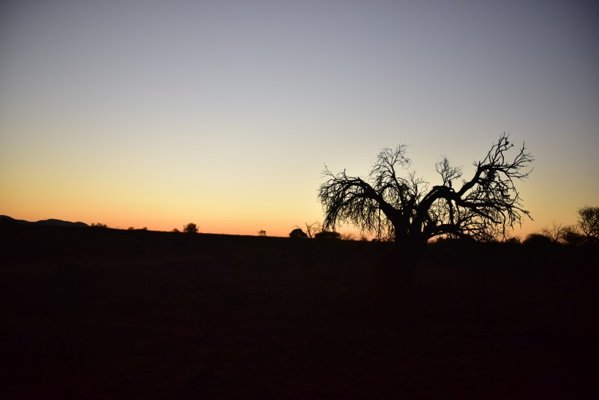
\includegraphics[width=1.\linewidth,height=0.88\linewidth]{images/qualitatives/evqa_name.jpg}
    \end{minipage}
    \hspace{0.02\linewidth}
    \begin{minipage}{0.7\linewidth}
        {
        \textbf{Q}: Controversy surrounds the origin of what in the city from which one would drive to reach this nature reserve? 
        \vspace{0.15cm}
        
        \textbf{Qwen2.5-VL-7B (ZS)~\cite{bai2025qwen2}}:\\
        Based on the information provided, the city from which one would drive to reach the nature reserve is Port Augusta West. The text mentions that Port Augusta West is a suburb of Port Augusta, South Australia, and lists it as the starting point for driving to the nature reserve \textcolor{red}{\xmark} \\
        \textbf{ReflectiVA~\cite{cocchi2025augmenting}}:\\
        The Town \textcolor{red}{\xmark} \\
        \textbf{\ours (Ours):}\\
       \texttt{<think>} The image shows a nature reserve with a tree silhouette against a sunset sky, which matches the setting described in the retrieved passages. The question specifically asks for the origin of something in a city from which one would drive to reach this particular nature reserve. None of the retrieved passages provide any relevant information whatsoever regarding the question asked. Therefore, the final logical is that these passages must be disregarded insofar as the question is concerned. \texttt{</think>} \texttt{<answer>} Willi Stoph \textcolor[HTML]{00b050}{\cmark} \texttt{</answer>} 
        }
    \end{minipage}
    \vspace{0.3cm}
\end{minipage}

\begin{minipage}{\linewidth}
    \begin{minipage}{0.3\linewidth} 
        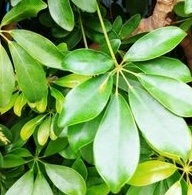
\includegraphics[width=1.\linewidth,height=0.88\linewidth]{images/qualitatives/evqa_pianta.jpg}
    \end{minipage}
    \hspace{0.02\linewidth}
    \begin{minipage}{0.7\linewidth}
        {
        \textbf{Q}: What genus are this plant and schefflera actinophylla in? \vspace{0.15cm}
        
        \textbf{Qwen2.5-VL-7B (ZS)~\cite{bai2025qwen2}}:\\
        Not enough information is provided to determine the genus in question \textcolor{red}{\xmark} \\
        \textbf{ReflectiVA~\cite{cocchi2025augmenting}}:\\
        Schefflera \textcolor{red}{\xmark} \\
        \textbf{\ours (Ours):}\\
       \texttt{<think>} The image shows a plant that matches the description of Schefflera actinophylla in the retrieved passage. The question specifically asks for the genus of this particular plant in the image and Schefflera actinophylla. Both plants are identified as belonging to the same genus in the retrieved passage. The question directly corresponds to the information presented in the retrieved passage without any need to refer to the other retrieved passages. Therefore, the final verdict is that the final question must ignore these retrieved passages entirely. \texttt{</think>} \texttt{<answer>} Heptapleurum \textcolor[HTML]{00b050}{\cmark} \texttt{</answer>} 
        }
    \end{minipage}
    \vspace{0.9cm}
\end{minipage}

\begin{minipage}{\linewidth}
    \begin{minipage}{0.3\linewidth}
        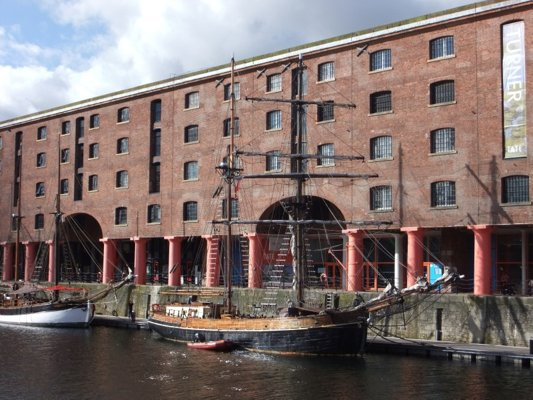
\includegraphics[width=1.\linewidth,height=0.88\linewidth]{images/qualitatives/sample_22_test_4_sample_4521_im_0.jpg}
    \end{minipage}
    \hspace{0.02\linewidth}
    \begin{minipage}{0.7\linewidth}
        {
        \textbf{Q}: Who designed this dock? \vspace{0.15cm}
        
        \textbf{Qwen2.5-VL-7B (ZS)~\cite{bai2025qwen2}}:\\
        Not enough information is provided to determine who designed the dock \textcolor{red}{\xmark} \\
        \textbf{ReflectiVA~\cite{cocchi2025augmenting}}:\\
        Jesse Hartley \textcolor{red}{\xmark} \\
        \textbf{\ours (Ours):}\\
       \texttt{<think>} The image shows the Albert Dock in Liverpool, which matches the question asked. The question specifically asks for the designer of this particular dock. The retrieved passage directly states that the dock in question, the Albert Dock, was designed by Jesse Hartley. Since the question specifically matches the dock in the image with the one mentioned in the passage, the retrieved passage directly answers the question without any need to refer to the question itself or the retrieved passage. \texttt{</think>} \texttt{<answer>} Royal Albert Dock \textcolor[HTML]{00b050}{\cmark} \texttt{</answer>} 
        }
    \end{minipage}
\end{minipage}
\vspace{-0.1cm}
\caption{Qualitative examples from Encyclopedic-VQA where we show the ability of \ours to reason about the question-image pair and the retrieved passages. For reference, we also report the generation from ReflectiVA~\cite{cocchi2025augmenting} and the corresponding zero-shot model.}
\label{fig:qualitatives_suppl_reasoning}
\end{figure*}


\begin{figure*}[t]
\begin{minipage}{0.325\linewidth}
\scriptsize{\textbf{Q}: What did the zuni people use the bark of this \\ plant to dye black?\vspace{0.05cm}}\\
\begin{minipage}{0.443\linewidth}
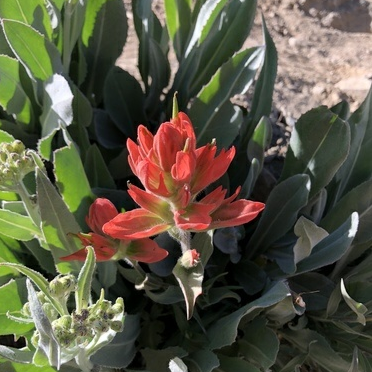
\includegraphics[width=1.\linewidth,height=0.88\linewidth]{images/qualitatives/EVQA_flower.png}
\end{minipage}
\hfill
\begin{minipage}{0.53\linewidth}
\scriptsize{
\textbf{Qwen2.5-VL-7B (ZS)~\cite{bai2025qwen2}}:\\
The plant you are referring to is the Desert Paintbrush [..] \textcolor{red}{\xmark} \\
\textbf{ReflectiVA~\cite{cocchi2025augmenting}}:\\
Dyes \textcolor{red}{\xmark} \\
\textbf{\ours (Ours):}\\
Deerskin \textcolor[HTML]{00b050}{\cmark}
}
\end{minipage}
\end{minipage}
\hspace{0.02cm}
\begin{minipage}{0.325\linewidth}
\scriptsize{\textbf{Q}: What type of hawksbeard is this plant \\ commonly known as? \vspace{0.05cm}}\\
\begin{minipage}{0.443\linewidth}
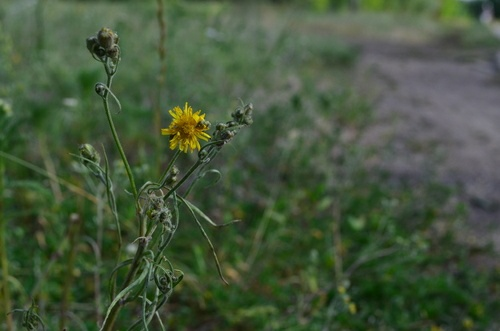
\includegraphics[width=1.\linewidth,height=0.88\linewidth]{images/qualitatives/EVQA_yellow_flower.png}
\end{minipage}
\hfill
\begin{minipage}{0.53\linewidth}
\scriptsize{
\textbf{Qwen2.5-VL-7B (ZS)~\cite{bai2025qwen2}}:\\
The plant in the image is likely rough hawksbeard \textcolor{red}{\xmark} \\
\textbf{ReflectiVA~\cite{cocchi2025augmenting}}:\\
Mouse-ear \textcolor{red}{\xmark} \\
\textbf{\ours (Ours):}\\
Narrowleaf \textcolor[HTML]{00b050}{\cmark}
}
\end{minipage}
\end{minipage}
\hspace{0.02cm}
\vspace{0.1cm}
\begin{minipage}{0.325\linewidth}
\scriptsize{\textbf{Q}: What did Alexander Wilson do to this bird in 1811?\vspace{0.05cm}}\\
\begin{minipage}{0.443\linewidth}
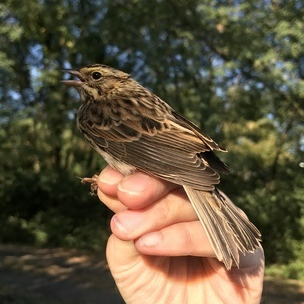
\includegraphics[width=1.\linewidth,height=0.88\linewidth]{images/qualitatives/EVQA_bird.png}
\end{minipage}
\hfill
\begin{minipage}{0.53\linewidth}
\scriptsize{
\textbf{Qwen2.5-VL-7B (ZS)~\cite{bai2025qwen2}}:\\
Alexander Wilson did not harm the bird in any way [..] \textcolor{red}{\xmark} \\
\textbf{ReflectiVA~\cite{cocchi2025augmenting}}:\\
I don't see any information about a bird species \textcolor{red}{\xmark} \\
\textbf{\ours (Ours):}\\
Discovered \textcolor[HTML]{00b050}{\cmark}
}
\end{minipage}
\end{minipage}

\begin{minipage}{0.325\linewidth}
\scriptsize{\textbf{Q}: What part of a tree is this plant often found under? \vspace{0.05cm}}\\
\begin{minipage}{0.443\linewidth}
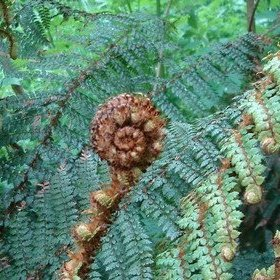
\includegraphics[width=1.\linewidth,height=0.88\linewidth]{images/qualitatives/sample_19_test_2_sample_2043_im_0.jpg}
\end{minipage}
\hfill
\begin{minipage}{0.53\linewidth}
\scriptsize{
\textbf{Qwen2.5-VL-7B (ZS)~\cite{bai2025qwen2}}:\\
Polystichum is often found under trees in disturbed habitats such as road cuts, talus slopes, and stream banks  \textcolor{red}{\xmark} \\
\textbf{ReflectiVA~\cite{cocchi2025augmenting}}:\\
Trunk \textcolor{red}{\xmark} \\
\textbf{\ours (Ours):}\\
Canopy \textcolor[HTML]{00b050}{\cmark}
}
\end{minipage}
\end{minipage}
\hspace{0.02cm}
\begin{minipage}{0.325\linewidth}
\scriptsize{\textbf{Q}: What monument was placed under state control in 1882? \vspace{0.05cm}}\\
\begin{minipage}{0.443\linewidth}
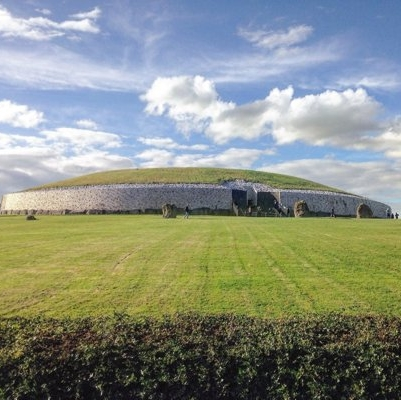
\includegraphics[width=1.\linewidth,height=0.88\linewidth]{images/qualitatives/sample_20_test_4_sample_4480_im_0.jpg}
\end{minipage}
\hfill
\begin{minipage}{0.53\linewidth}
\scriptsize{
\textbf{Qwen2.5-VL-7B (ZS)~\cite{bai2025qwen2}}:\\
Newgrange was placed under state control in 1882 \textcolor{red}{\xmark} \\
\textbf{ReflectiVA~\cite{cocchi2025augmenting}}:\\
Newgrange \textcolor{red}{\xmark} \\
\textbf{\ours (Ours):}\\
Newgrange and Knowth and Dowth \textcolor[HTML]{00b050}{\cmark}
}
\end{minipage}
\end{minipage}
\hspace{0.02cm}
\vspace{0.1cm}
\begin{minipage}{0.325\linewidth}
\scriptsize{\textbf{Q}: What type of habitat does this plant prefer?\vspace{0.05cm}}\\
\begin{minipage}{0.443\linewidth}
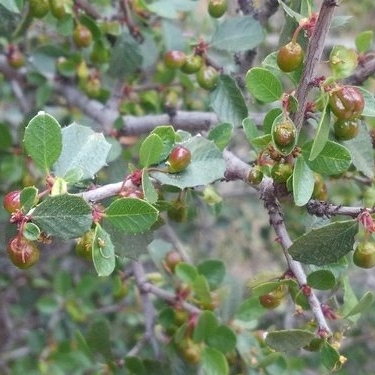
\includegraphics[width=1.\linewidth,height=0.88\linewidth]{images/qualitatives/sample_18_test_2_sample_2123_im_0.jpg}
\end{minipage}
\hfill
\begin{minipage}{0.53\linewidth}
\scriptsize{
\textbf{Qwen2.5-VL-7B (ZS)~\cite{bai2025qwen2}}:\\
It cannot be determined from the given information alone, but it is likely to [..] \textcolor{red}{\xmark} \\
\textbf{ReflectiVA~\cite{cocchi2025augmenting}}:\\
Dry \textcolor{red}{\xmark} \\
\textbf{\ours (Ours):}\\
Chaparral \textcolor[HTML]{00b050}{\cmark}
}
\end{minipage}
\end{minipage}

\begin{minipage}{0.325\linewidth}
\scriptsize{\textbf{Q}: In what german city is this landmark the most famous?\vspace{0.05cm}}\\
\begin{minipage}{0.443\linewidth}
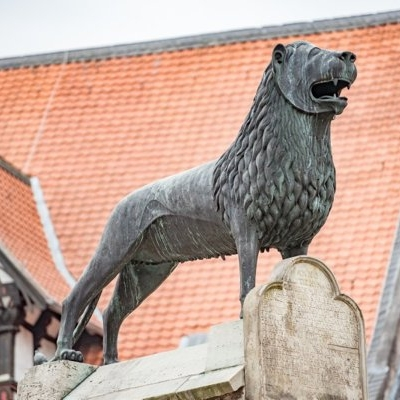
\includegraphics[width=1.\linewidth,height=0.88\linewidth]{images/qualitatives/sample_17_test_2_sample_2634_im_0.jpg}
\end{minipage}
\hfill
\begin{minipage}{0.53\linewidth}
\scriptsize{
\textbf{Qwen2.5-VL-7B (ZS)~\cite{bai2025qwen2}}:\\
The landmark in the picture is the Brunswick Lion \textcolor{red}{\xmark} \\
\textbf{ReflectiVA~\cite{cocchi2025augmenting}}:\\
Braunschweig \textcolor{red}{\xmark} \\
\textbf{\ours (Ours):}\\
Brunswick \textcolor[HTML]{00b050}{\cmark}
}
\end{minipage}
\end{minipage}
\hspace{0.02cm}
\begin{minipage}{0.325\linewidth}
\scriptsize{\textbf{Q}: What is the habitat of this animal? \vspace{0.05cm}}\\
\begin{minipage}{0.443\linewidth}
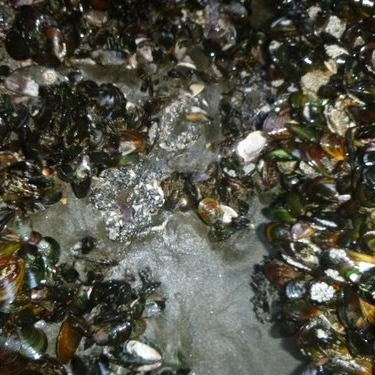
\includegraphics[width=1.\linewidth,height=0.88\linewidth]{images/qualitatives/sample_16_test_0_sample_482_im_0.jpg}
\end{minipage}
\hfill
\begin{minipage}{0.53\linewidth}
\scriptsize{
\textbf{Qwen2.5-VL-7B (ZS)~\cite{bai2025qwen2}}:\\
In the upper intertidal zone on open coast [..] \textcolor{red}{\xmark} \\
\textbf{ReflectiVA~\cite{cocchi2025augmenting}}:\\
Salt marshes and quiet bays \textcolor{red}{\xmark} \\
\textbf{\ours (Ours):}\\
Intertidal zone on the open coast \textcolor[HTML]{00b050}{\cmark}
}
\end{minipage}
\end{minipage}
\hspace{0.02cm}
\vspace{0.1cm}
\begin{minipage}{0.325\linewidth}
\scriptsize{\textbf{Q}: Which teams played against each other in the first match ever held in this stadium? \vspace{0.05cm}}\\
\begin{minipage}{0.443\linewidth}
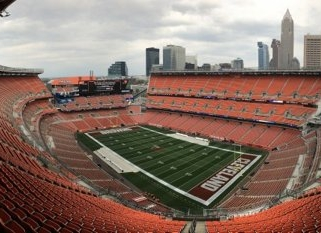
\includegraphics[width=1.\linewidth,height=0.88\linewidth]{images/qualitatives/sample_15_test_0_sample_957_im_0.jpg}
\end{minipage}
\hfill
\begin{minipage}{0.53\linewidth}
\scriptsize{
\textbf{Qwen2.5-VL-7B (ZS)~\cite{bai2025qwen2}}:\\
The first match ever held in FirstEnergy Stadium, [..] \textcolor{red}{\xmark} \\
\textbf{ReflectiVA~\cite{cocchi2025augmenting}}:\\
Minnesota vikings \textcolor{red}{\xmark} \\
\textbf{\ours (Ours):}\\
Browns and Minnesota Vikings \textcolor[HTML]{00b050}{\cmark}
}
\end{minipage}
\end{minipage}

\begin{minipage}{0.325\linewidth}
\scriptsize{\textbf{Q}: What type of bird is the Contopus cooperi? \vspace{0.05cm}}\\
\begin{minipage}{0.443\linewidth}
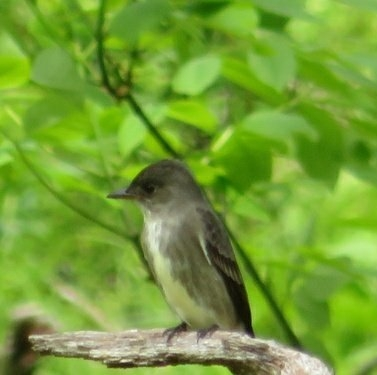
\includegraphics[width=1.\linewidth,height=0.88\linewidth]{images/qualitatives/sample_14_test_1_sample_1424_im_0.jpg}
\end{minipage}
\hfill
\begin{minipage}{0.53\linewidth}
\scriptsize{
\textbf{Qwen2.5-VL-7B (ZS)~\cite{bai2025qwen2}}:\\
Contopus cooperi (Olive-sided Flycatcher) \textcolor{red}{\xmark} \\
\textbf{ReflectiVA~\cite{cocchi2025augmenting}}:\\
Passerine \textcolor{red}{\xmark} \\
\textbf{\ours (Ours):}\\
Flycatcher \textcolor[HTML]{00b050}{\cmark}
}
\end{minipage}
\end{minipage}
\hspace{0.02cm}
\begin{minipage}{0.325\linewidth}
\scriptsize{\textbf{Q}: What month of meteorological winter in the northern hemisphere did hungary purchase this building? \vspace{0.05cm}}\\
\begin{minipage}{0.443\linewidth}
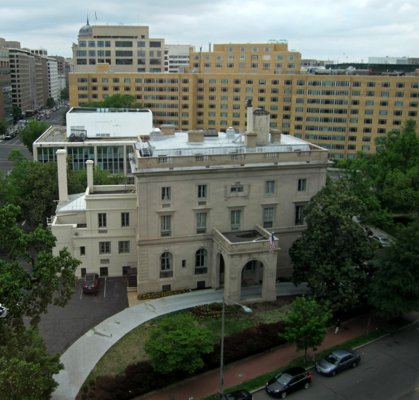
\includegraphics[width=1.\linewidth,height=0.88\linewidth]{images/qualitatives/sample_13_test_5_sample_5336_im_0.jpg}
\end{minipage}
\hfill
\begin{minipage}{0.53\linewidth}
\scriptsize{
\textbf{Qwen2.5-VL-7B (ZS)~\cite{bai2025qwen2}}:\\
According to the information provided, the U.S. Civil Service Building was built [..] in 1911 \textcolor{red}{\xmark} \\
\textbf{ReflectiVA~\cite{cocchi2025augmenting}}:\\
December \textcolor{red}{\xmark} \\
\textbf{\ours (Ours):}\\
Third \textcolor[HTML]{00b050}{\cmark}
}
\end{minipage}
\end{minipage}
\hspace{0.02cm}
\vspace{0.1cm}
\begin{minipage}{0.325\linewidth}
\scriptsize{\textbf{Q}: What wars ended the year the fichtelberg cable car was built on this mountain? \vspace{0.05cm}}\\
\begin{minipage}{0.443\linewidth}
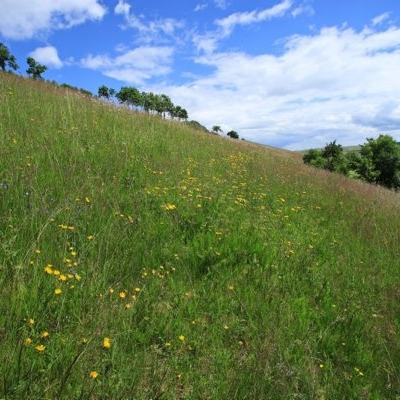
\includegraphics[width=1.\linewidth,height=0.88\linewidth]{images/qualitatives/sample_12_test_5_sample_5397_im_0.jpg}
\end{minipage}
\hfill
\begin{minipage}{0.53\linewidth}
\scriptsize{
\textbf{Qwen2.5-VL-7B (ZS)~\cite{bai2025qwen2}}:\\
Not enough information is provided to determine [..] \textcolor{red}{\xmark} \\
\textbf{ReflectiVA~\cite{cocchi2025augmenting}}:\\
World war i \textcolor{red}{\xmark} \\
\textbf{\ours (Ours):}\\
The American Indian Wars \textcolor[HTML]{00b050}{\cmark}
}
\end{minipage}
\end{minipage}

\begin{minipage}{0.325\linewidth}
\scriptsize{\textbf{Q}: Who dies without a male heir in the netherlands the year this plant was introduced to canada? \vspace{0.05cm}}\\
\begin{minipage}{0.443\linewidth}
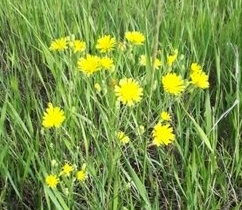
\includegraphics[width=1.\linewidth,height=0.88\linewidth]{images/qualitatives/sample_11_test_5_sample_5210_im_0.jpg}
\end{minipage}
\hfill
\begin{minipage}{0.53\linewidth}
\scriptsize{
\textbf{Qwen2.5-VL-7B (ZS)~\cite{bai2025qwen2}}:\\
Queen Beatrix \textcolor{red}{\xmark} \\
\textbf{ReflectiVA~\cite{cocchi2025augmenting}}:\\
The dutch royal family \textcolor{red}{\xmark} \\
\textbf{\ours (Ours):}\\
King William III \textcolor[HTML]{00b050}{\cmark}
}
\end{minipage}
\end{minipage}
\hspace{0.02cm}
\begin{minipage}{0.325\linewidth}
\scriptsize{\textbf{Q}: Who was the duke of milan when Edward Cowper began leading the monks at this abbey? \vspace{0.05cm}}\\
\begin{minipage}{0.443\linewidth}
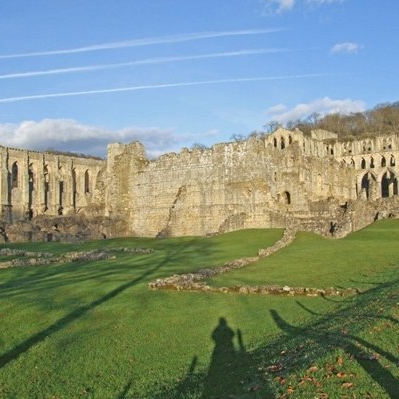
\includegraphics[width=1.\linewidth,height=0.88\linewidth]{images/qualitatives/sample_10_test_5_sample_5506_im_0.jpg}
\end{minipage}
\hfill
\begin{minipage}{0.53\linewidth}
\scriptsize{
\textbf{Qwen2.5-VL-7B (ZS)~\cite{bai2025qwen2}}:\\
The Duke of Brittany, William de Lis, was the owner of the patronage of Roche Abbey \textcolor{red}{\xmark} \\
\textbf{ReflectiVA~\cite{cocchi2025augmenting}}:\\
Charles i \textcolor{red}{\xmark} \\
\textbf{\ours (Ours):}\\
Maximilian Sforza \textcolor[HTML]{00b050}{\cmark}
}
\end{minipage}
\end{minipage}
\hspace{0.02cm}
\vspace{0.1cm}
\begin{minipage}{0.325\linewidth}
\scriptsize{\textbf{Q}: For what football cup final is this stadium the venue? \vspace{0.05cm}}\\
\begin{minipage}{0.443\linewidth}
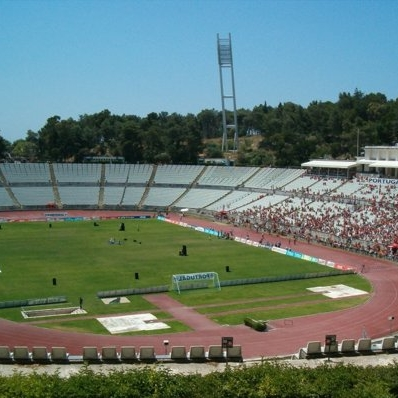
\includegraphics[width=1.\linewidth,height=0.88\linewidth]{images/qualitatives/sample_2_test_2_sample_2789_im_0.jpg}
\end{minipage}
\hfill
\begin{minipage}{0.53\linewidth}
\scriptsize{\textbf{Qwen2.5-VL-7B (ZS)~\cite{bai2025qwen2}}:\\
The football cup final for which this stadium is the venue is the Taça de Portugal \textcolor{red}{\xmark} \\
\textbf{ReflectiVA~\cite{cocchi2025augmenting}}:\\
Uefa women's championship \textcolor{red}{\xmark} \\
\textbf{\ours (Ours):}\\
Portuguese \textcolor[HTML]{00b050}{\cmark}
}
\end{minipage}
\end{minipage}

\begin{minipage}{0.325\linewidth}
\scriptsize{\textbf{Q}: In what month does it not snow in this lake? \vspace{0.05cm}}\\
\begin{minipage}{0.443\linewidth}
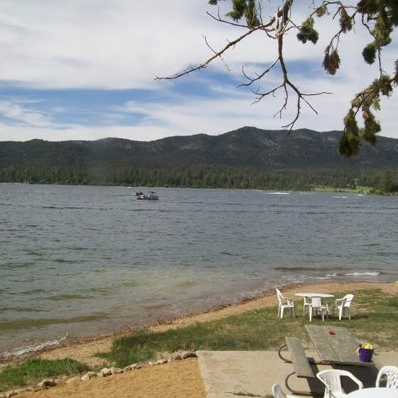
\includegraphics[width=1.\linewidth,height=0.88\linewidth]{images/qualitatives/sample_1_test_4_sample_4659_im_0.jpg}
\end{minipage}
\hfill
\begin{minipage}{0.53\linewidth}
\scriptsize{
\textbf{Qwen2.5-VL-7B (ZS)~\cite{bai2025qwen2}}:\\
The lake is not affected by snowfall, [..] \textcolor{red}{\xmark} \\
\textbf{ReflectiVA~\cite{cocchi2025augmenting}}:\\
July \textcolor{red}{\xmark} \\
\textbf{\ours (Ours):}\\
July and August \textcolor[HTML]{00b050}{\cmark}
}
\end{minipage}
\end{minipage}
\hspace{0.02cm}
\begin{minipage}{0.325\linewidth}
\scriptsize{\textbf{Q}: What is the religious order of this monastery? \vspace{0.05cm}}\\
\begin{minipage}{0.443\linewidth}
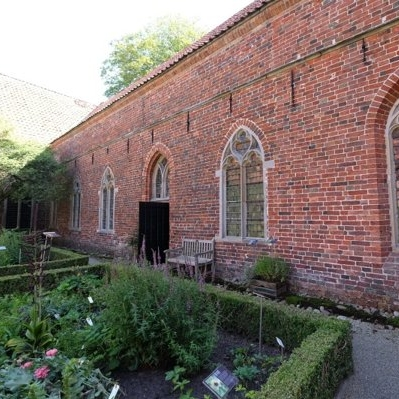
\includegraphics[width=1.\linewidth,height=0.88\linewidth]{images/qualitatives/sample_3_test_0_sample_703_im_0.jpg}
\end{minipage}
\hfill
\begin{minipage}{0.53\linewidth}
\scriptsize{
\textbf{Qwen2.5-VL-7B (ZS)~\cite{bai2025qwen2}}:\\
Bremian Knighthood \textcolor{red}{\xmark} \\
\textbf{ReflectiVA~\cite{cocchi2025augmenting}}:\\
Premonstratensian \textcolor{red}{\xmark} \\
\textbf{\ours (Ours):}\\
 Order of the Holy Cross \textcolor[HTML]{00b050}{\cmark}
}
\end{minipage}
\end{minipage}
\hspace{0.02cm}
\vspace{0.1cm}
\begin{minipage}{0.325\linewidth}
\scriptsize{\textbf{Q}: What is the surface area of this lake? \vspace{0.05cm}}\\
\begin{minipage}{0.443\linewidth}
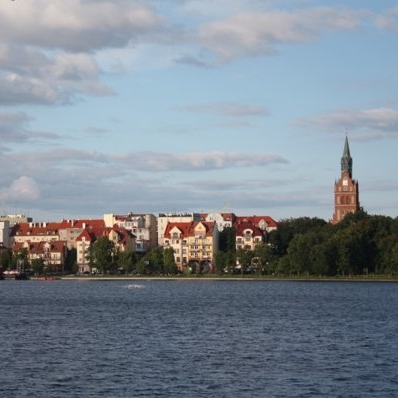
\includegraphics[width=1.\linewidth,height=0.88\linewidth]{images/qualitatives/sample_4_test_0_sample_653_im_0.jpg}
\end{minipage}
\hfill
\begin{minipage}{0.53\linewidth}
\scriptsize{
\textbf{Qwen2.5-VL-7B (ZS)~\cite{bai2025qwen2}}:\\
Ełk Lake is a fresh water lake in the Masurian Lake District of Poland's Warmia-Mazury Province \textcolor{red}{\xmark} \\
\textbf{ReflectiVA~\cite{cocchi2025augmenting}}:\\
3.82 \textcolor{red}{\xmark} \\
\textbf{\ours (Ours):}\\
3.82 square kilometres \textcolor[HTML]{00b050}{\cmark}
}
\end{minipage}
\end{minipage}

\begin{minipage}{0.325\linewidth}
\scriptsize{\textbf{Q}: Who designed this palace?
 \vspace{0.05cm}}\\
\begin{minipage}{0.443\linewidth}
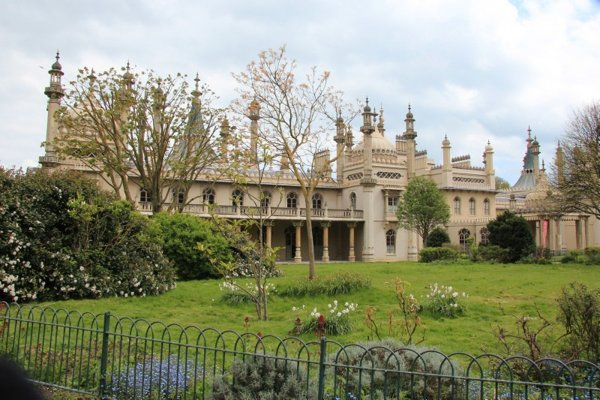
\includegraphics[width=1.\linewidth,height=0.88\linewidth]{images/qualitatives/sample_25_test_0_sample_799_im_0.jpg}
\end{minipage}
\hfill
\begin{minipage}{0.53\linewidth}
\scriptsize{
\textbf{Qwen2.5-VL-7B (ZS)~\cite{bai2025qwen2}}:\\
Not enough information is provided to determine [..]  \textcolor{red}{\xmark} \\
\textbf{ReflectiVA~\cite{cocchi2025augmenting}}:\\
Peter Frederick Robinson \textcolor{red}{\xmark} \\
\textbf{\ours (Ours):}\\
John Nash \textcolor[HTML]{00b050}{\cmark}
}
\end{minipage}
\end{minipage}
\hspace{0.02cm}
\begin{minipage}{0.325\linewidth}
\scriptsize{\textbf{Q}: In which country or region does this animal live?
 \vspace{0.05cm}}\\
\begin{minipage}{0.443\linewidth}
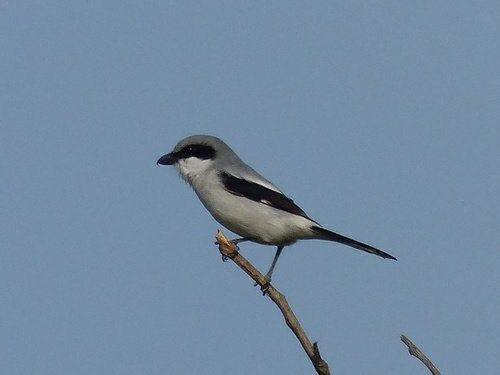
\includegraphics[width=1.\linewidth,height=0.88\linewidth]{images/qualitatives/sample_24_test_0_sample_414_im_0.jpg}
\end{minipage}
\hfill
\begin{minipage}{0.53\linewidth}
\scriptsize{
\textbf{Qwen2.5-VL-7B (ZS)~\cite{bai2025qwen2}}:\\
It is native to southern Canada, the contiguous USA, and Mexico \textcolor{red}{\xmark} \\
\textbf{ReflectiVA~\cite{cocchi2025augmenting}}:\\
Eurasia \textcolor{red}{\xmark} \\
\textbf{\ours (Ours):}\\
North America \textcolor[HTML]{00b050}{\cmark}
}
\end{minipage}
\end{minipage}
\hspace{0.02cm}
\vspace{0.1cm}
\begin{minipage}{0.325\linewidth}
\scriptsize{\textbf{Q}: How many eggs does this bird typically lay? \vspace{0.05cm}}\\
\begin{minipage}{0.443\linewidth}
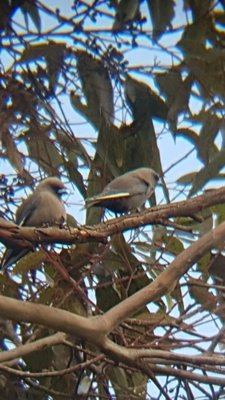
\includegraphics[width=1.\linewidth,height=0.88\linewidth]{images/qualitatives/sample_23_test_0_sample_430_im_0.jpg}
\end{minipage}
\hfill
\begin{minipage}{0.53\linewidth}
\scriptsize{
\textbf{Qwen2.5-VL-7B (ZS)~\cite{bai2025qwen2}}:\\
Three eggs \textcolor{red}{\xmark} \\
\textbf{ReflectiVA~\cite{cocchi2025augmenting}}:\\
Three \textcolor{red}{\xmark} \\
\textbf{\ours (Ours):}\\
Three to four \textcolor[HTML]{00b050}{\cmark}
}
\end{minipage}
\end{minipage}

\vspace{-0.25cm}
\caption{Qualitative results on InfoSeek and Encyclopedic-VQA image-question pairs comparing \ours, ReflectiVA~\cite{cocchi2025augmenting}, and the corresponding zero-shot model.}
\label{fig:qualitatives_suppl}
\vspace{-0.35cm}
\end{figure*}
